\chapter{Dataset}
In this chapter we will describe in detail, what simulations did we run and how we proceeded with the automated temperature fitting to obtain the dataset for surrogate temperature modelling.
\section{EPOCH Simulations}
The EPOCH simulation was run in following setting:
\begin{itemize}
	\item The intensities of the laser: $I=10^{17}\,\mathrm{W.cm}^{-2}$, $I=10^{18} \,\mathrm{W.cm}^{-2}$ and \newline$I=10^{19}\,\mathrm{W.cm}^{-2}$.
	\item The angle of incidence with respect to target normal direction: \newline $\alpha \in \{0\degree,1\degree,2\degree,3\degree,4\degree,5\degree,10\degree,20\degree,30\degree,40\degree,45\degree,50\degree,60\degree\}$.
	\item The characteristic scale length of the preplasma: \newline $L\in\{0.01,0.02,0.05,0.1,0.2,0.5,1,2,5\}$ in microns.
	\item The laser wavelength is 1 micron.
	\item The laser is p-polarized and focused to a Gaussian spot of size $3.2$ mircons.
	\item The density in the target ranges from about $0.01n_c$ to $3.\gamma_{osc}n_c$, where $n_c$ is critical density of laser radiation \cite{cui2013} and $\gamma_{osc}$ is defined in \cite{cui2013}.
	\item The initial temperature of plasma is 100 eV.
	\item The target is composed of electrons and protons. They are represented by 30 macro-particles per cell.
	\item They are represented by 30 macro-particles per cell. The resolution of spatial grid is 33nm and the time step satisfies the CFL condition \cite{arber2015}.
	
\end{itemize}
The simulations have been performed on the Q3 node of the Quantum Hyperion cluster at FNSPE. The input file that used to start the EPOCH simulation can be seen in appendix \ref{att:input-deck}.

\section{Temperature fitting}
The results of the simulations are transformed into histograms as it was described in chapter \ref{ch:temp-fitting-theory}. We fixed the histogram size to 1000 bins with their width scaling with the maximum electron energy.

Before fitting the data, it is essential to prepare it appropriately. In practice, this involves removing a few bins in the beginning and several bins in the end of the electron energy spectrum. The lower energy bins can be removed, because they do not contribute to hot electrons temperature very much. Also, they can contain error, as the low energy electrons need more time to reach the virtual detector and the simulation can end before that happens. This step ensures that the analysis focuses on the relevant and meaningful parts of the spectrum.

The histogram \ref{fig:example-histogram} after the cut-off can be seen in figure \ref{fig:trimmed-hist}.

\begin{figure}[h]
	\centering
	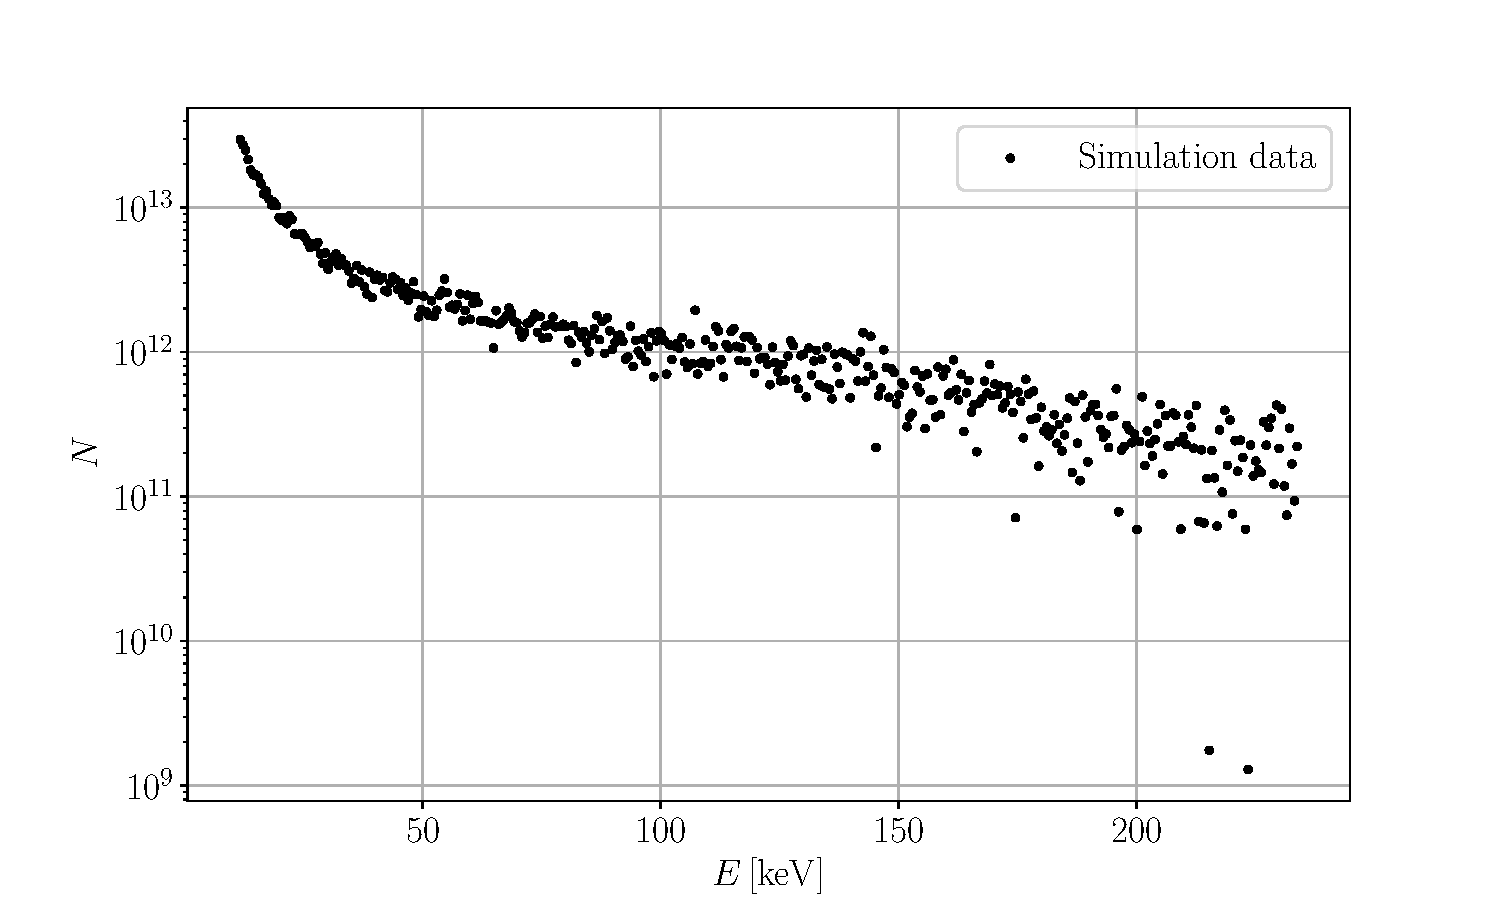
\includegraphics[width=0.8\textwidth]{figures/trimmed-hist}
	\caption{An example of trimmed histogram with simulation parameters $I=10^{19}\,\mathrm{W.cm}^{-2}$, $L=0.1\,\mathrm{\mu m}$ and $\alpha = 10$°.}
	\label{fig:trimmed-hist}
\end{figure}

The Jacquelin method was implemented in programming language python as a class with number of exponential terms as a parameter. However, the lack of the numerical stability for more exponential term discussed at the end of chapter \ref{ch:temp-fitting-theory} usually causes issues for more than three terms.
